\documentclass[a4paper]{article}

\usepackage{natbib}
\usepackage{INTERSPEECH_v2}
\usepackage[utf8]{inputenc} % allow utf-8 input
\usepackage[T1]{fontenc}    % use 8-bit T1 fonts
\usepackage[draft]{hyperref}       % hyperlinks
\usepackage{url}            % simple URL typesetting
\usepackage{booktabs}       % professional-quality tables
\usepackage{amsfonts}       % blackboard math symbols
\usepackage{nicefrac}       % compact symbols for 1/2, etc.
\usepackage{microtype}      % microtypography

\usepackage{amsmath,graphicx}
\usepackage{bm}
\usepackage{url}
\usepackage{amsmath}
\usepackage{amsthm}
\usepackage{graphicx}
\usepackage{subcaption}
\usepackage{algorithm2e}
\usepackage{pbox}
\usepackage{multirow}
\errorcontextlines 10000

\title{Adversarial Training of Invariant Features for Speech Recognition}
\name{Dmitriy Serdyuk$^1$, Kartik Audhkhasi$^2$, 
      Bhuvana Ramabhadran$^2$, Phil\'emon Brakel$^1$, Samuel Thomas$^2$,
      Yoshua Bengio$^{1\dagger}$}
\address{
  $^1$MILA, Universit\'e de Montr\'eal, Canada\\
  $^2$IBM Watson, USA\\
  $^\dagger$CIFAR Fellow}
\email{serdyuk@iro.umontreal.ca}

\begin{document}

\maketitle
% 
\begin{abstract}
Recent advances in domain adaptation allow us to construct networks that are
invariant to certain labeled factors. The reverse gradient algorithm uses an
adversarial learning approach to train a network to produce the desired label
as well as to deceive a second classifier that is trained on adaptation 
labels. This is tightly connected to the ideas behind generative adversarial 
networks (GANs). Therefore, some insights for training GANs are needed for the
reverse gradient's successful application. We adapt this approach to train an 
acoustic system that is invariant to undesirable factors such as the recording
environment noise type. We conduct experiments on a popular dataset.
\end{abstract}
\noindent\textbf{Index Terms}: speech recognition, adversarial training, 
reverse gradient
\section{Introduction}
\label{sec:intro}
    One of the most challenging aspects of automatic speech recognition (ASR)
    is the mismatch between the training and testing acoustic conditions. 
    During testing, a system may encounter new recording conditions, 
    microphone types, speakers, accents and types of background noises. 
    Furthermore, even if the test scenarios are seen during training, there 
    can be significant variability in their statistics. Thus, it's important to 
    develop ASR systems that are invariant to unseen acoustic conditions.

    Several model and feature based adaptation methods such as Maximum 
    Likelihood Linear Regression (MLLR),  feature-based MLLR and 
    i-vectors~\citep{saon2013speaker} have been proposed to handle speaker 
    variability; and Noise Adaptive Training \citep[NAT;][]{kalinli2010noise}
    and Vector Taylor Series \citep[VTS;][]{un1998speech} to handle 
    environment variability.
    % The end-to-end part has become sort of irrelevant given that the
    % experiments are actually with hybrid systems and this version of the paper will not
    % have to be sold as being end-to-end anymore.
    With the increasing success of Deep Neural 
    Network~(DNN) acoustic models for ASR investigated 
    in~\citep{hinton2012deep,seide2011conversational,sainath2011making}, 
    and in more recent works~\citep{miao2015eesen,sainath2015learning} 
    complicated structure of acoustic conditions is modeled within a single network.
    This allows us to take 
    advantage of the network's ability to learn highly non-linear feature 
    transformations, with greater flexibility in constructing training 
    objective functions that promote learning of noise invariant 
    representations.
    % Phil: The part below should include speaker invariance and mention the WSJ task
    The main idea of this work is to force the acoustic model 
    to learn a representation which is invariant to noise conditions, instead of 
    explicitly using noise robust acoustic features 
    (Section~\ref{sec:invariant-speech}). This type of noise-invariant 
    training requires noise-condition labels during training only. It is 
    related to the idea of generative adversarial networks (GAN) and the 
    gradient reverse method proposed by~\cite{goodfellow2014generative} 
    and~\cite{ganin2014unsupervised} respectively 
    (Section~\ref{sec:background}). Then we discuss previous work in 
    Section~\ref{sec:relatedwork}. 
    We present results on the Aurora-4 speech 
    recognition task in Section~\ref{sec:experiments} and summarize 
    our findings in Section~\ref{sec:discussion}.

\section{Background}
\label{sec:background}
\begin{figure*}
    \centering

    \captionsetup[subfigure]{oneside,margin={0.3cm,0cm}}
    \begin{subfigure}[b]{0.49\linewidth}
    \centering
        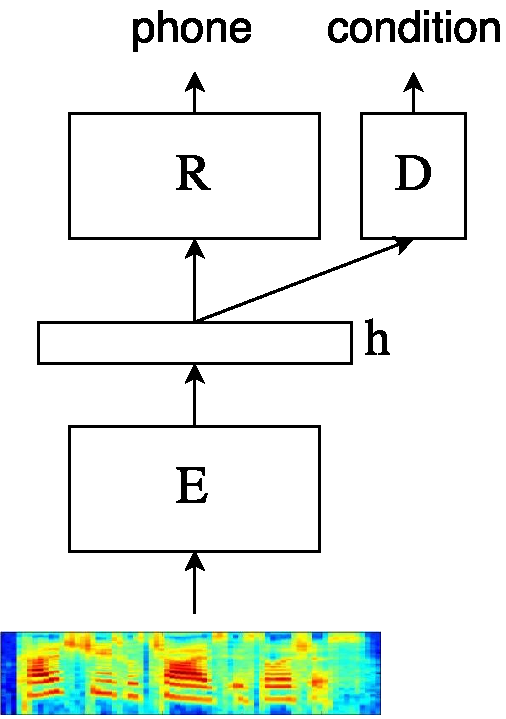
\includegraphics[width=0.4\linewidth]{model.pdf}
        \caption{The model consists of three neural networks. The encoder $E$ produces
        the intermediate representation $h$ which used in the recognizer $R$ and 
        in the domain discriminator $D$. The hidden representation $h$ is trained to improve
        the recognition and minimize the domain discriminator accuracy. The domain discriminator
        is a classifier trained to maximize its accuracy on the noise type
        classification task.}
        \label{fig:model}
    \end{subfigure}
    \begin{subfigure}[b]{0.5\linewidth}
        \centering
        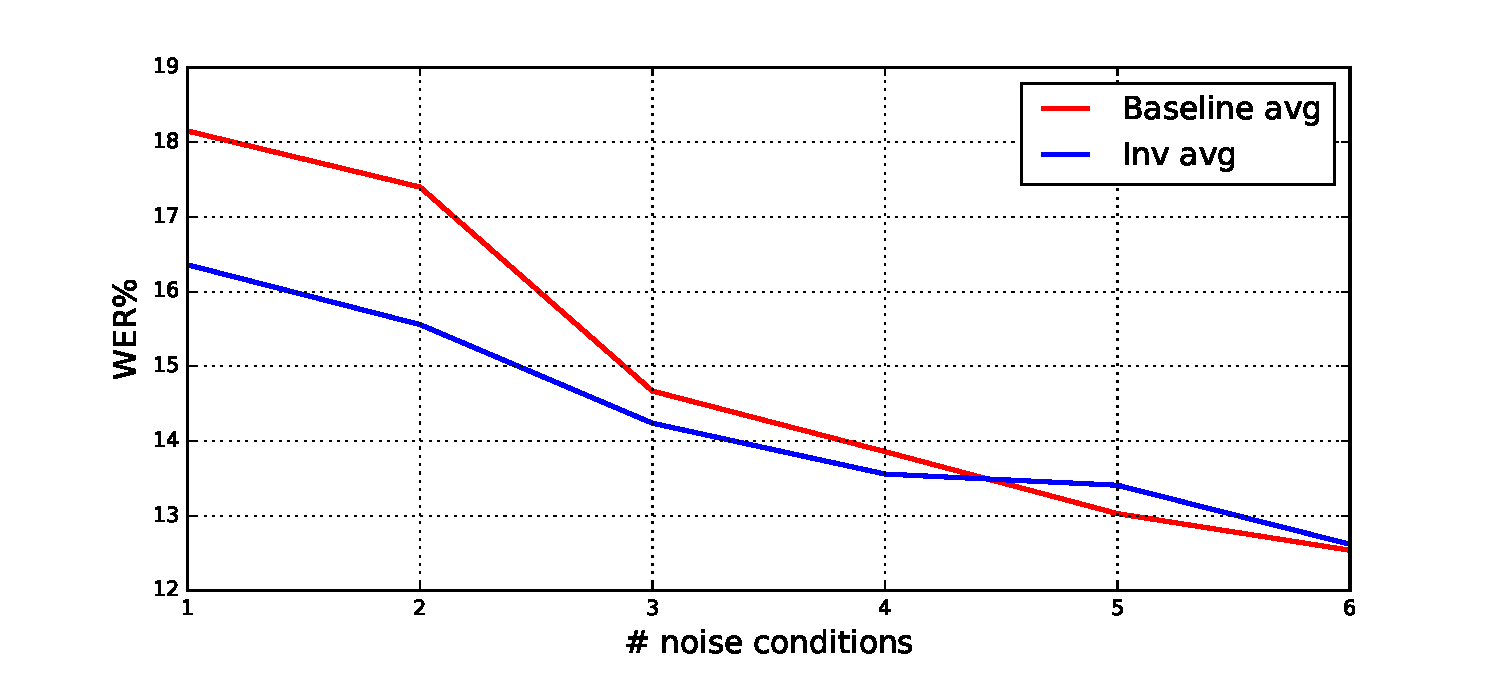
\includegraphics[width=0.7\linewidth]{wer_avg.pdf}
        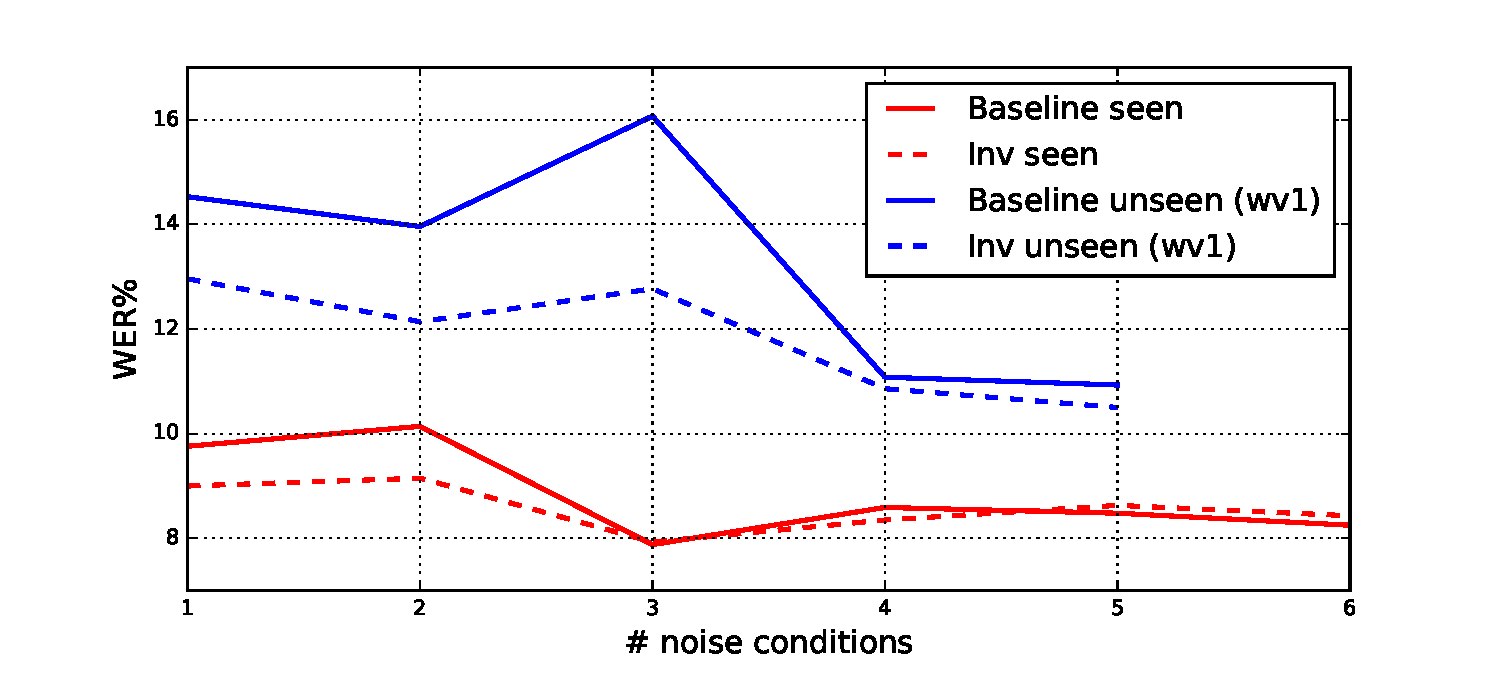
\includegraphics[width=0.7\linewidth]{wer_seen_unseen.pdf}
        \caption{Top: Average performance of the baseline multi-condition and invariance model varying with  the number of noise
            conditions used for training. Bottom: Average performance on seen versus unseen noise conditions.
            Testing was performed on all wv1 conditions (Sennheiser microphone).
            }
        \label{fig:results}
    \end{subfigure}
    \caption{The model and summarized results.}
\end{figure*}
\emph{Generative Adversarial Networks} consist of two networks: the generator and the discriminator. 
    The generator network $G$ has an
    input of randomly-generated feature vectors and is asked to produce a
    sample, e.g.\ an image, similar to the images in the training set. The discriminator network $D$
    can either receive a generated image from the generator $G$ or an image
    from the training set. Its task is to distinguish
    between the ``counterfeit'' generated image and the ``genuine'' image taken from the dataset. Thus,
    the discriminator is just a classifier network with a sigmoid output layer
    and can be trained with gradient back-propagation. This gradient can be propagated further
    to the generator network (assuming that the output of the generator is
    continuous).

    The two networks in the GAN setup are competing with each other: the 
    generator is trying to deceive the discriminator network, while the discriminator tries
    to do its best to recognize if there was a deception, similar to adversarial game-theoretic settings.    
    Formally, the objective function of GAN training is
    \begin{align}
        \min_G \max_D V(D, G) = &\mathbb{E}_{\bm{x} \sim p_{\text{data}}(\bm{x})}[\log D(\bm{x})] + \\
            &\mathbb{E}_{\bm{z} \sim p_{\bm{z}}(\bm{z})}[\log (1 - D(G(\bm{z})))].
        \label{eq:gan}
    \end{align}
    The maximization over the discriminator $D$ forms a usual cross-entropy objective, the gradients are
    computed with respect to the parameters of $D$. An important property of
    this objective is that the gradient of the composition~$D(G(\cdot))$ is well
    defined. Therefore the generator~$G$ can be trained with the back-propagation
    algorithm using the gradient signal from the discriminator~$D$.
    The generator~$G$ is
    minimizing the classification objective using the gradients
    propagated through the second term. The minimization over $G$ makes it
    produce samples which $D$ classifies as originating from the train data.

    Several practical guidelines were proposed for optimizing GANs by~\cite{radford2015unsupervised} and 
    further explored by~\cite{salimans2016improved}. The second term of Eq.~\ref{eq:gan}
    is frequently exchanged with
    \begin{equation}
        - \mathbb{E}_{\bm{z} \sim p_{\bm{z}}(\bm{z})}[\log (D(G(\bm{z})))].
    \end{equation}
    The gradient of this term has the same sign but it has better properties.
    We experimented with several losses for our discriminator and chose one
    similar to Eq.~\ref{eq:gan} but we maintain the negative sign in our notation
    to demonstrate the general direction of the gradient of the discriminator loss.

    %TODO
    % dima: I want to add something like this:
    %Another point of view on the GAN training is that the generator is matching
    %the distribution of the data with the distribution of the generator using
    %a discriminator to provide the training signal. This approach can be generalized
    %on any distributions to be matched.
    Optimization of the GAN objective corresponds to a minimization of the
    so-called Jenson-Shannon divergence between the data distribution and the
    distribution represented by the generator. This divergence is zero if and
    only if the two distributions are identical. From this perspective, we can
    say that the discriminator provides a training signal which allows
    one to match distributions in general. In this work we are interested in
    matching feature distributions of different noise conditions.

    Prior work by~\cite{ganin2014unsupervised} proposed a method for training a network 
    which can be adapted to new domains. The training data consists of the images
    labeled with classes of interest and separate domain (image background) labels. 
    The network has a $Y$-shaped structure: the image is fed to the
    first network which produces a hidden representation $h$. Then this 
    representation $h$ is input to two separate networks: a domain classifier network ($D$) and 
    a target classifier network ($R$). The goal of training is to learn a hidden 
    representation that is invariant to the domain labels and still performs well on 
    the target classification task, so that the domain information doesn't 
    interfere with the target classifier at test time. Similar to the GAN 
    objective, which forces the generation distribution be close to the data distribution,
    the \emph{gradient reverse method} makes domain specific distributions similar to each other.

    The network is trained with three goals: the hidden representation $h$ should
    be helpful for the target classifier, harmful for the domain classifier,
    and the domain classifier should have a good classification accuracy. More 
    formally, the authors define the loss function as
    \begin{equation}
        L = L_1(\hat{y}, y; \theta_R, \theta_E) + 
        \alpha L_2(\hat{d}, d; \theta_D) -
        \beta L_3(\hat{d}, d; \theta_E),
        \label{eq:grm}
    \end{equation}
    where $y$ is the ground truth class, $d$ is the domain label, corresponding
    hat variables are the network predictions, and $\theta_E, \theta_R$ and 
    $\theta_D$ are the subsets of  parameters for the encoder,
    recognizer and the domain classifier networks respectively. The hyper-parameters
    $\alpha$ and $\beta$ denote the relative influence of the loss functions terms.

\section{Related Work}
\label{sec:relatedwork}
    Neural networks display some robustness towards different recording
    conditions and speaker by themselves and the effectiveness of representations
    produced by a neural network for internal 
    noise reduction is discussed by~\cite{yu2013feature}. This work sets a 
    baseline for experiments on the Aurora-4 dataset.

    To be even more robust with respect to different recording conditions and speakers,
    one can either aim to adapt the model parameters to these new situations or
    to learn representations which are invariant to them.
    Most approaches so far, are based on adaptation.
    Unfortunately, many of the adaptation methods which have been designed for
    GMM-HMM systems cannot be applied to DNN-based systems. For this reason, a
    large body of recent work has investigated new adaptation methods for neural
    networks.

    Some of the linear and affine transformations used for GMM adaptation can
    still be applied to neural networks when one limits these adaptations to the
    very last layer, as was shown in~\cite{yao2012adaptation}. The
    improvements seemed to rely mostly on the adaptation of the bias parameters.
    A clear downside of this approach is that it doesn't utilize the
    representational power provided by the non-linear multi-layer structure of deep
    neural networks.

    Many neural network speaker adaptation methods are based on
    i-vectors. The most common way to exploit i-vectors is by providing them as additional
    inputs~\citep{senior2014improving,saon2013speaker}. This means that i-vectors also need to
    be available during testing and this may not always be practical.

    In the specific case of noise robustness, one can use speech enhancement to
    obtain more robust features and neural networks have been used for this for
    decades~\citep{knecht1995neural}. A further step in this direction is to train
    systems to recognize speech and perform speech enhancement jointly~\citep{narayanan2014joint}. 
    We argue that speech enhancement is a more difficult task to learn than
    invariance to certain noise conditions and more likely to suffer from
    overfitting when the amount of available noisy data is limited.
    Another downside of enhancement approaches is that there is no reason to
    expect them to generalize well to noise conditions that were not available during
    training.

    Another adaptation strategy is to retrain the model parameters using a very small
    number of utterances from the new domain while making sure that the model
    doesn't stray too far away from the parameter values that were obtained from
    the train data~\citep{yu2013kl}.
    The adaptation to new domains can also be kept under control by limiting
    the number of parameters which are adapted to the new data or by limiting the
    adaptation to a rescaling of the hidden unit activations~\citep{swietojanski2014learning}.
    The most important difference between these approaches and our work is that
    we don't adapt the model parameters at all after training. In many
    situations this may not be possible and retraining of models may require more
    from the hardware on which the speech recognition system is implemented.

    Recently, in a work by~\cite{yusuke2016adversarial} a multi-layer sigmoidal network was trained 
    in an adversarial fashion on an in-house transcription task corrupted by noise.
    This work is very similar to our approach but we evaluate our methods on
    more challenging benchmark while investigating different numbers of noise
    conditions. Our work also differs due to the use of more modern rectifier
    activation based classification networks.
    Finally, in other very recent work~\citep{saon2017english} a form of adversarial training with a network
    that predicts an i-vector using the mean square error loss was used.

\section{Invariant Representations for Speech Recognition}
\label{sec:invariant-speech}

Most ASR systems are DNN-HMM hybrid systems. The context dependent (CD) HMM 
states (acoustic model) are the class labels of interest. The
recording conditions, speaker identity, or gender represent the domains in 
GANs. The task is to make the hidden layer representations of the HMM state classifier network 
invariant with respect to these domains. We hypothesize that this adversarial method of
training helps the HMM state classifier to generalize better to unseen domain conditions and requires only a  
small additional amount of supervision, i.e., the domain labels.  

Figure~\ref{fig:model} depicts the model, which is same as the model for the 
gradient reverse method. It is a feed-forward neural network trained to predict 
the CD-HMM state, with a branch that predicts the domain (noise condition). This 
branch is discarded in the testing phase. In our experiments we
used the noise condition as the domain label, merging all noise types into one label
and defining `clean' as the other label. Our training loss function is Eq.~\ref{eq:grm} with 
$L_3$ set to $d\log(1 - \hat{d}) + (1-d)\log(\hat{d})$ for stability during training. 
$L_3$ term maximizes the probability
of an incorrect domain classification in contrast to the gradient reverse where the 
correct classification is minimized.
The terms $L_1$ and $L_2$ are 
regular cross-entropies which are minimized with corresponding parameters $\theta_E$ and $\theta_D$.
For simplicity, we use only a single hyper-parameter -- the weight of the third term.

\begin{table*}[t]
    \centering
    \caption{Average word error rates (WER\%) on Aurora-4 dataset on all test conditions,
        including seen and unseen noise and unseen microphone. The first column
        specifies the number of noise conditions used for the training. The
        results in the last row are from a preliminary experiment with
        layer-wise pre-training, close to state-of-the-art
        model and a corresponding invariance training starting with a pretrained model.}
    \label{tab:results}
    \begin{tabular}{r|cc||cc|cc|cc|cc}
    %\multirow{2}{*}{Subset} & \multicolumn{2}{c}{Orig}  & \multicolumn{2}{|c}{Inv}\\ 
    %           & wv1  & wv2  & wv1  & wv2 \\
        Noise       &Inv&BL&  \multicolumn{2}{c|}{A} & \multicolumn{2}{c|}{B} & \multicolumn{2}{c|}{C} & \multicolumn{2}{c}{D}\\
               & & &  Inv & BL & Inv & BL & Inv & BL & Inv & BL\\
    \hline
    1           &16.36        &18.14 &6.54&7.57    &12.71& 14.09   & 11.45&   13.10    & 22.47 &   24.80    \\
    2           &15.56        &17.39 &5.90&  6.58 &   11.69   &13.28   &11.12   &13.51   &21.79   &23.96 \\
    3           &14.24        &14.67 &5.45 & 5.08&    10.76&   12.44&   9.75&    9.84 &   19.93&   19.30\\
    4           &13.61        &13.84 & 5.08 &5.29    &9.73    &9.97    &9.49    &9.56    &19.49   &19.90\\         
    5           &13.41        &13.02 & 5.12 &5.34    &9.52    &9.42    &9.55    &8.67    &19.33   &18.65\\         
    6           &12.62        &12.60 & 4.80 &4.61    &9.04    &8.86    &8.76    &8.59    &18.16   &18.21\\
    \hline\hline
    6* &11.85        &11.99    &4.52    &4.76    &8.76    &8.76    &7.79    &8.57    &16.84&    16.99
    \end{tabular}
\end{table*}

\section{Experiments}
\label{sec:experiments}
We experimentally evaluated our approach   
on the well-benchmarked Aurora-4 \citep{parihar2002aurora} noisy speech recognition task. Aurora-4
is based on the Wall Street Journal corpus (WSJ0). It contains noises of 
six categories which were added to the clean data. Every clean and noisy
utterance has been 
% TODO!!!!
% what kind of frequency characteristics?
filtered to simulate the phone quality recording using P.341 \citep{parihar2002aurora}. The training
data contains 4400 clean utterances and 446 utterances for each noise condition,
i.e., a total of 2676 noisy utterances.
The test set consists of clean data, data corrupted by 6 noise types, and data 
recorded with a different microphone for both the clean and noisy conditions.

For both the clean and noisy data, we extracted 40-dimensional Mel-filterbank features with their deltas and 
delta-deltas spliced over $\pm$5 frames, resulting in 1320 input 
features that were subsequently mean and variance normalized. The baseline
acoustic model was a 6-layer 
DNN with 2048 rectified linear units at every layer. It was trained using 
momentum-accelerated stochastic gradient descent for 15 epochs with new-bob 
annealing~\citep[the learning rate is halfed if no improvement on the validation set, as in][]{morgan1995continuous,sainath2011making}.

To evaluate the impact of our method on generalization to \emph{unseen} noises (the
most typical situation in practice),
we performed 6 experiments with different sets of noises seen during training.
The networks were trained
on clean data, with each noise condition added one-by-one in the following order: airport, babble, car, 
restaurant, street, and train. The last training group included all noises and therefore matched the
standard multi-condition training setup. For every training group, we trained the
baseline and the invariance model, where we branched out at the $4^{th}$ layer to a
binary classifier predicting clean versus noisy data. Due to the imbalance between amounts of clean and
noisy utterances, we had to oversample noisy frames to ensure that every mini-batch contained
equal number of clean and noisy speech frames.

Table~\ref{tab:results} summarizes the results. Figure~\ref{fig:results} visualizes 
the word error rate (WER) for the baseline multi-condition training and invariance training 
as the number of seen noise types varies. We conclude that the best performance
gain is achieved when a small number of noise types are available during training. 
It can be seen that invariance training is able to generalize better to unseen 
noise types compared with multi-condition training.
In practice, it's only possible to train on a small fraction of all the possible
noise conditions in the world, so this apparent ability to generalize to unseen
conditions is a promising result.
% dima: we need to add that this is good news and very reasonable

We note that our experiments did not use layer-wise pre-training, commonly used for small
datasets. The baseline WERs reported are very close to the state-of-the-art. 
Our preliminary experiments on a pre-trained network (better overall WER) when 
using all noise types (last row of Table~\ref{tab:results}) for training show 
the same trend as the non-pretrained networks.

\section{Discussion}
\label{sec:discussion}
    This paper presents the application of generative adversarial networks and 
    invariance training for noise robust speech recognition. We show that invariance training 
    helps the ASR system to generalize better to unseen noise conditions and improves 
    the word error rate when a small number of noise types are seen during training. Our 
    experiments show that in contrast to the image recognition task, in speech 
    recognition, the domain adaptation network suffers from underfitting. Therefore, the 
    gradient of the $L_3$ term in Eq.~\ref{eq:grm} is unreliable and noisy. Future 
    research includes enhancements to the domain adaptation network while exploring 
    alternative network architectures and invariance-promoting loss functions.

\section{Acknowledgments}

We would like to thank Yaroslav Ganin, David Warde-Farley for insightful discussions,
developers of Theano~\citep{theano2016theano}, Blocks, and Fuel~\citep{MerrienboerBDSW15} 
for great toolkits. 
The authors would like to acknowledge the support of the following agencies for
research funding and computing support: NSERC, Calcul Qu\'{e}bec, Compute Canada,
the Canada Research Chairs and CIFAR. Dmitriy Serdyuk thanks Samsung for partial
financial support of this work.

\bibliographystyle{IEEEtranN}

\bibliography{refs}
\end{document}
